\documentclass[11pt]{article}
\usepackage{latexsym}
\usepackage{natbib}
\usepackage{graphicx}
\usepackage{caption}
\usepackage{subcaption}
\usepackage{listings}
\usepackage{algorithm}
\usepackage{algpseudocode}

\title{Homework 4: Approximate Inference in Bayesian Networks}
\author{Shun Zhang}
\date{}

\begin{document}
\maketitle

\section{Sampling Methods}

In this assignment, I implemented Rejection Sampling and Gibbs
Sampling to generate samples for a Bayesian network. 

For Rejection Sampling, the implementation is quite simple. Samples
are generated ignoring the constraints of the evidence. Then, samples
inconsistent with the evidence are dropped. In the remaining samples,
proportion of samples consistent with the query is returned.

For Gibbs Sampling, in each iteration, for node $x_i$, it is sampled
from the following probability (revised from the textbook).

\begin{equation}
p(x_i|x_{\{j \not = i\}}) \propto \prod_k P(x_k|pa_k)
\end{equation}

\section{Experiments}

\begin{figure}
\centering
\begin{subfigure}[b]{0.49\textwidth}
	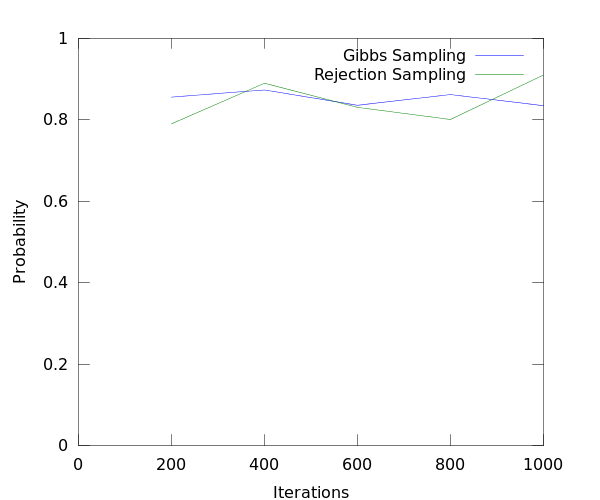
\includegraphics[width=\textwidth]{ian1.png}
	\caption{$P(X_0=1 | E_1) $}
	\end{subfigure}
\begin{subfigure}[b]{0.49\textwidth}
	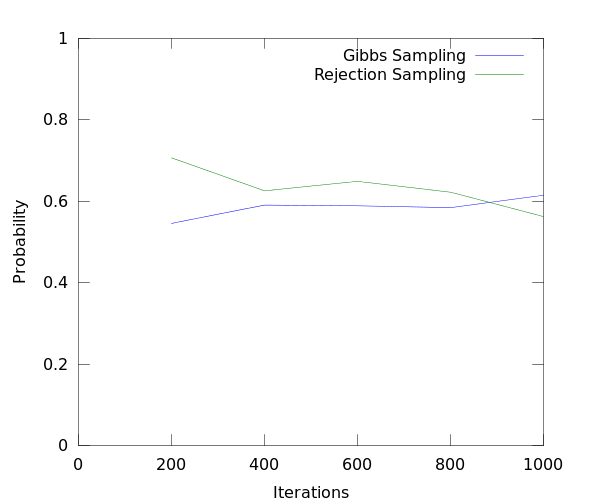
\includegraphics[width=\textwidth]{ian2.png}
	\caption{$P(X_1=1 | E_1) $}
\end{subfigure}
\begin{subfigure}[b]{0.49\textwidth}
	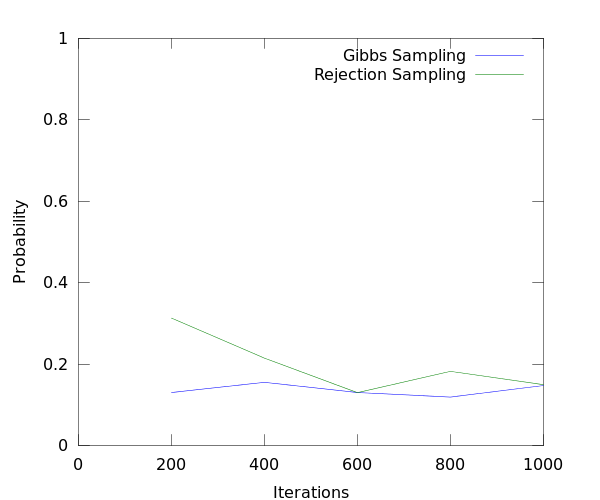
\includegraphics[width=\textwidth]{ian3.png}
	\caption{$P(X_2=1 | E_1) $}
\end{subfigure}
\begin{subfigure}[b]{0.49\textwidth}
	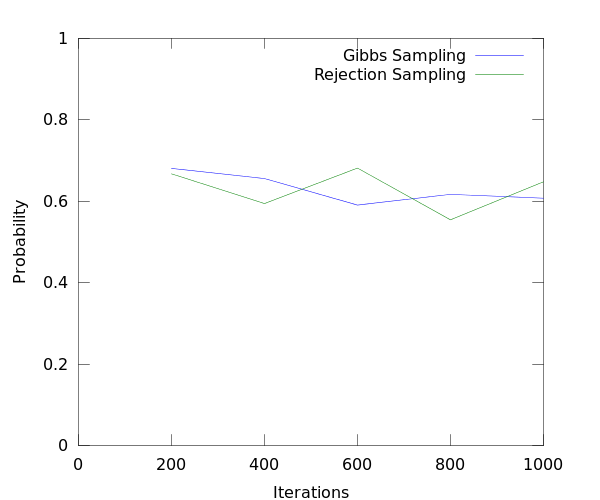
\includegraphics[width=\textwidth]{ian4.png}
	\caption{$P(X_3=1 | E_1) $}
\end{subfigure}
\begin{subfigure}[b]{0.49\textwidth}
	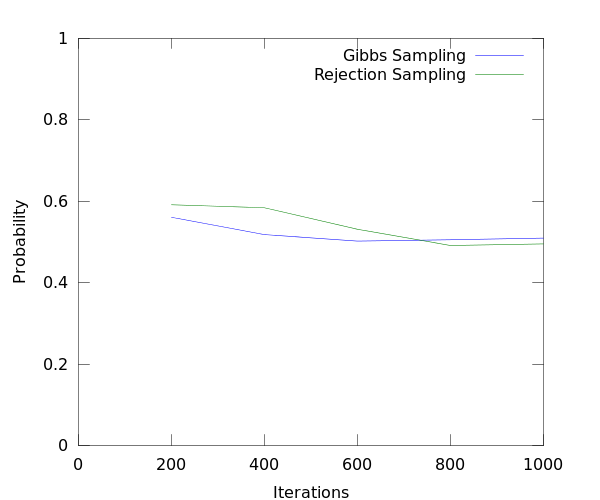
\includegraphics[width=\textwidth]{ian5.png}
	\caption{$P(X_4=1 | E_1) $}
\end{subfigure}
\begin{subfigure}[b]{0.49\textwidth}
	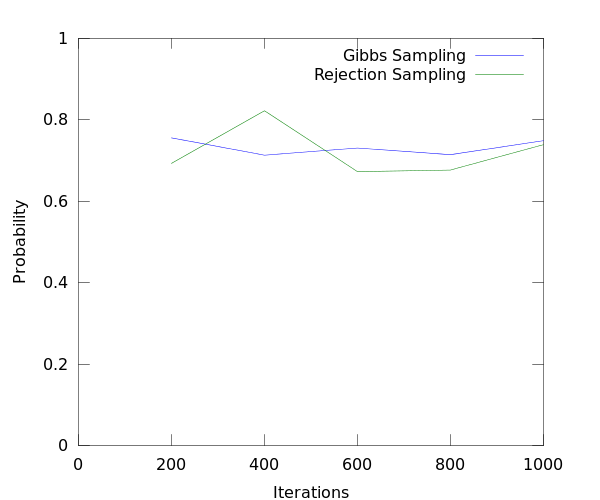
\includegraphics[width=\textwidth]{ian6.png}
	\caption{$P(X_5=1 | E_1) $}
\end{subfigure}
\caption{Sampling process for each test case. $E_1$ denotes $(X_6 = 1,
X_7 = 0, X_8 = 0)$.}
\label{fig:lp}
\end{figure}

In this experiment, I used the data provided by Ian. The results
generated are shown below.

In Figure~\ref{fig:lp}, I show the learning process in each sampling
algorithms, for each query data for the first envidence given.

\end{document}
